\documentclass[a4paper,12pt,twocolumn]{article}

\usepackage{times}
\usepackage[utf8]{inputenc}
\usepackage[brazil]{babel}
\usepackage[a4paper,margin=2cm,columnsep=1cm]{geometry}
\usepackage{authblk}
\usepackage{titlesec}
\usepackage[pdftex]{graphicx}
\usepackage{mathtools}
\usepackage{amsmath}
\usepackage{enumitem}
\usepackage[font={footnotesize}]{caption}
\usepackage{bm}


\topmargin      0.0cm
\headheight     0.0cm
\headsep        0.0cm
\oddsidemargin  0.0cm
\evensidemargin 0.0cm
\textheight     22.86cm
\textwidth      16.51cm

\graphicspath{{images/}}
\titleformat*{\section}{\normalsize\bfseries\filcenter}
\titleformat*{\subsection}{\normalsize\bfseries\filcenter}

\renewcommand{\figurename}{\small Figure}
\newcommand{\figureref}[1]{Fig. (\ref{fig:#1})}
\newcommand{\equationref}[1]{Eq. (\ref{eq:#1})}
\newcommand{\bigsum}{\displaystyle\sum}
\newcommand{\twopartdef}[4]
{
    \left\{
        \begin{array}{ll}
            #1 & \mbox{se } #2 \\
            #3 & \mbox{se } #4
        \end{array}
    \right.
}
\newcommand{\tworowsmatrix}[2]
{
    \begin{bmatrix}
            #1\\
            #2
    \end{bmatrix}
}


\begin{document}

\title{\textbf{Resumo de Aprendizagem de Máquina 2014-2}}
\author{
    \textbf{Eduardo M. B. de A. Tenório}\\
    \small{\texttt{embat@cin.ufpe.br}}
}
\affil{\large CIn-UFPE}
\date{}

\maketitle


\begin{abstract}
\begin{itshape}
Este documento tem por finalidade ser um resumo dos assuntos abordados na disciplina \emph{Aprendizagem de Máquina} do período 2014-2 do CIn-UFPE, ministrada pelos professores Francisco Carvalho e Teresa Ludermir. A maioria do documento referencia o livro ``Pattern Classification", de Duda, Hart \& Stork. Os códigos utilizados como exercício de fixação encontram-se em \normalfont{github.com/embatbr/resumo-aprendizagem}.
\end{itshape}
\end{abstract}


\section{Teoria da Decisão Bayesiana}

\subsection{Introdução}

Teoria da Decisão Bayesiana é uma abordagem estatística para a classificação de
padrões, baseada em quantificar os tradeoffs associados a tomar uma determinada
decisão (classificar) utilizando probabilidade e considerando os custos associados.

O \textbf{estado natural} é denotado por $\omega$, de modo que $\omega = \omega_i$, para $i = 1, 2, ..., c$, significa que o exemplo foi classificado como pertencente à classe $\omega_i$. Cada uma dessas classes possui uma \textbf{probabilidade a priori} $P(\omega_i)$, com

\begin{equation}
    \sum_{i=1}^{c} P(\omega_i) = 1,
    \label{eq:sum_priori_prob_to_one}
\end{equation}

\noindent refletindo o conhecimento prévio da chance de um elemento da classe $\omega_i$ aparecer. A \textbf{regra de decisão} fica:

\begin{equation}
    \text{Decida } \omega_i \text{ se } i = \arg\max_j P(\omega_j).
    \label{eq:decision_1}
\end{equation}

\noindent Neste caso a classe $\omega_i$ sempre é escolhida e a probabilidade de erro é dada por:

\begin{equation}
    P_{err}(\omega_i) = 1 - P(\omega_i).
    \label{eq:prob_i_error}
\end{equation}

Utilizando uma característica $x$ que seja contínua e aleatória, sua \textbf{densidade de probabilidade estado-condicional} é dada por $p(x|\omega)$. Logo, a diferença entre $p(x|\omega_i)$ e $p(x|\omega_j)$ descreve a diferença da característica $x$ entre as populações das classes $\omega_i$ e $\omega_j$.

\begin{figure}[ht]
    \centering
    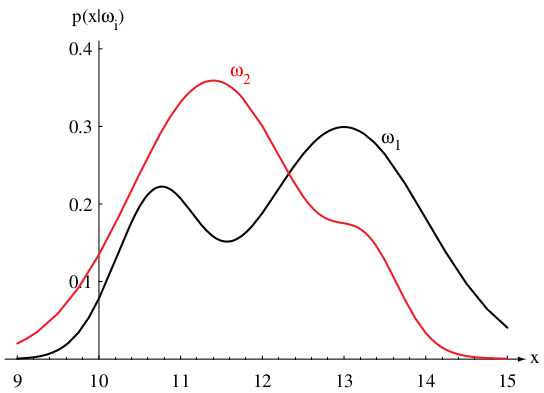
\includegraphics[width=\columnwidth]{state-conditional_pdf}
    \caption{Para $\omega_i = \omega_2$, é mais frequente observar $x$ entre 11 e 12 que $x = 13$ (valor mais provável se $\omega_i = \omega_1$).}
    \label{fig:state-conditional_pdf}
\end{figure}

Sabendo $P(\omega_i)$ e $p(x|\omega_i)$, e medindo um valor $x$, a probabilidade conjunta de achar um padrão na classe $\omega_i$ e com $x$ é dado por: $p(\omega_i,x) = P(\omega_i|x)p(x) = p(x|\omega_i)P(\omega_i)$, que pela \textbf{fórmula de Bayes} fica:

\begin{equation}
    P(\omega_i|x) = \frac{p(x|\omega_i)P(\omega_i)}{p(x)},
    \label{eq:bayes}
\end{equation}

\noindent com a evidência para $c$ classes
\begin{equation}
    p(x) = \sum_{j=1}^c p(x|\omega_j)P(\omega_j).
    \label{eq:bayes}
\end{equation}

A probabilidade a posteriori das classes $\omega_1$ e $\omega_2$ para um conjunto de valores de $x$ é mostrada em \figureref{posteriori_prob}. A regra de decisão fica:
\begin{equation}
    \text{Decida } \omega_i \text{ se } i = \arg\min_j P(erro_j|x),
    \label{eq:decision_2}
\end{equation}

\noindent onde
\begin{equation}
    P(erro_i|x) = \sum_{j\neq i} P(\omega_j|x),
    \label{eq:bayes}
\end{equation}

\noindent ou simplesmente $P(erro_i|x) = 1 - P(\omega_i|x)$. Então a regra torna-se:
\begin{equation}
    \text{Decida } \omega_i \text{ se } i = \arg\max_j P(\omega_j|x),
    \label{eq:decision_3}
\end{equation}

\begin{figure}[ht]
    \centering
    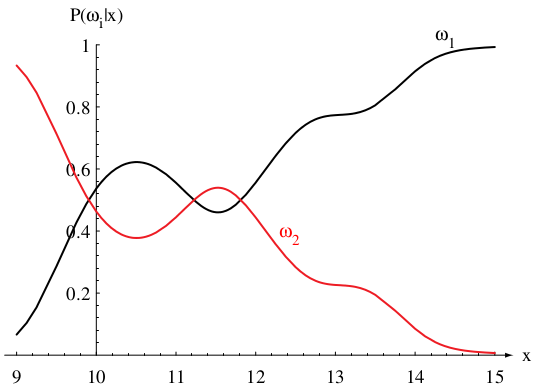
\includegraphics[width=\columnwidth]{posteriori_prob}
    \caption{Probabilidades a posteriori para $P(\omega_1) = \frac{2}{3}$ e $P(\omega_2) = \frac{1}{3}$, e para as densidades de probabilidade estado-condicional mostradas em \figureref{state-conditional_pdf}.}
    \label{fig:posteriori_prob}
\end{figure}

Esta regra minimiza a probabilidade média de erro, dada por
\begin{equation}
    P(erro_i) = \int_{-\infty}^{\infty} P(erro_i|x)p(x) dx.
    \label{eq:bayes}
\end{equation}

\subsection{Características Contínuas}

É de fácil compreensão que a característica $x$ pode ser trocada por um vetor de características $\boldsymbol{x} = (x_1, x_2, ..., x_d)$, onde $\boldsymbol{x}$ pertence ao espaço $\boldsymbol{R}^d$ (espaço de características). A região que decide $\omega_i$ é denotada por $\mathcal{R}_i$.

Outras ações além de apenas classificar um elemento podem ser tomadas, como por exemplo a \textbf{rejeição}: recusar-se a tomar uma decisão; uma opção válida quando o custo de ser indeciso é aceitável. Para isso \textbf{funções de custo} são inseridas, permitindo tratar de situações onde alguns erros de classificação são mais importantes que outros.

Seja $\{\omega_1, ..., \omega_c\}$ o conjunto finito de $c$ classes e seja $\{\alpha_1, ..., \alpha_a\}$ o conjunto finito de possíveis ações. A função de custo $\lambda(\alpha_i|\omega_j)$ descreve o custo de tomar a ação $\alpha_i$ quando a classe é $\omega_j$. Logo, observado um $\boldsymbol{x}$ em particular, tomar a ação $\alpha_i$ quando a classe é $\omega_j$ leva a um custo esperado (\textbf{risco})
\begin{equation}
    R(\alpha_i|\boldsymbol{x}) = \sum_{j=1}^c \lambda(\alpha_i|\omega_j) P(\omega_j|\boldsymbol{x}).
    \label{eq:conditional_risk}
\end{equation}

$R(\alpha_i|\boldsymbol{x})$ é chamado de \textbf{risco condicional}. Qualquer que seja o $\boldsymbol{x}$ observado, o risco pode ser minimizado selecionando a ação que minimiza $R(\alpha_i|\boldsymbol{x})$.

A regra de decisão geral é uma função $\alpha(\boldsymbol{x})$ que diz qual ação tomar para cada possível observação, ou seja, para cada $\boldsymbol{x}$ a \textbf{função de decisão} $\alpha(\boldsymbol{x})$ assume um dos $a$ valores $\alpha_1, ..., \alpha_a$.
\begin{equation}
    \alpha(\boldsymbol{x}) = \alpha_i \text{ se } i = \arg\min_j R(\alpha_j|\boldsymbol{x}),
    \label{eq:decision_4}
\end{equation}

\noindent Logo, o \textbf{risco global} é dado por

\begin{equation}
    R = \int R(\alpha(\boldsymbol{x}))p(\boldsymbol{x})d\boldsymbol{x}.
    \label{eq:conditional_risk}
\end{equation}

O risco global mínimo é chamado de \textbf{risco de Bayes}, denotado por $R^*$, sendo a melhor perfomance alcançável.

\subsection{Taxa de Erro Mínima}

Para evitar erros, a regra de decisão procurada é aquela que minimiza a probabilidade de erro, i.e. minimiza a \textbf{taxa de erro}. A função de custo de interesse para este caso é chamada de \textbf{simétrica} ou \textbf{zero-um},

\begin{equation}
    \lambda(\alpha_i|\omega_j) = \twopartdef{0}{i=j}{1}{i \neq j}
    \label{eq:loss_zero_one}
\end{equation}

\noindent para $i, j = 1, ..., c$. Como todos os erros tem custo igual, o risco condicional é dado por

\begin{equation}
    R(\alpha_i|\boldsymbol{x}) = 1 - P(\omega_i|\boldsymbol{x})
    \label{eq:conditional_risk_zero_one}
\end{equation}

\noindent com $P(\omega_i|\boldsymbol{x})$ sendo a probabilidade condicional da ação $\alpha_i$ estar correta. A regra de decisao neste caso continua:
\begin{equation}
    \text{Decida } \omega_i \text{ se } i = \arg\max_j P(\omega_j|x).
    \label{eq:decision_5}
\end{equation}

\begin{figure}[ht]
    \centering
    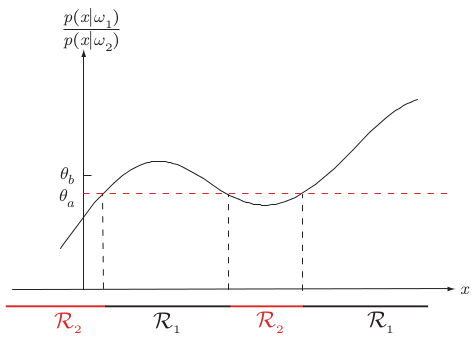
\includegraphics[width=\columnwidth]{decision_region}
    \caption{Se a penalização de classificar $\omega_1$ como $\omega_2$ for maior que o oposto, então a razão tende ao threshold $\theta_b$.}
    \label{fig:decision_region}
\end{figure}

\subsection{Funções Discriminantes}

A maneira mais usual de representar classificadores de padrões é através de um conjunto de \textbf{funções discriminantes} $g_i(\boldsymbol{x}), i = 1, ..., c$. O classificador atribui um vetor de características $\boldsymbol{x}$ à classe $\omega_i$ se

\begin{figure}[ht]
    \centering
    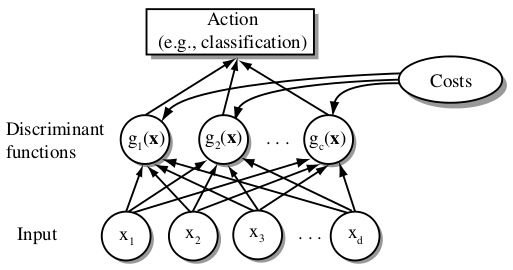
\includegraphics[width=\columnwidth]{discriminant_functions}
    \caption{Classificador com $c$ funções discriminantes e entradas $d$-dimensional. A ação geralmente é ``escolher o maior $g_i(\boldsymbol{x})$".}
    \label{fig:discriminant_functions}
\end{figure}

\begin{equation}
    g_i(\boldsymbol{x}) = \arg\max_j g_j(\boldsymbol{x})
    \label{eq:discriminant_functions}
\end{equation}

Para o caso geral com riscos, pode-se fazer $g_i(\boldsymbol{x}) = - R(\alpha_i|\boldsymbol{x})$, enquanto para o caso ``taxa de erro mínima", $g_i(\boldsymbol{x}) = P(\omega_i|\boldsymbol{x})$. A função discriminante $g_i(\boldsymbol{x})$ pode ser substituída por $f(g_i(\boldsymbol{x}))$, com $f(\cdot)$ sendo uma função monotonicamente crescente (e.g. logaritmo), com o resultado da classificação ficando inalterado. Como resultado, $\boldsymbol{R}^d$ é dividido em regiões de decisão $\mathcal{R}_i$ (não necessariamente conectadas) para cada classe $\omega_i$.

Para o caso em que $c = 2$, o classificador é chamado \textbf{dicotomizador}, e apenas uma função discriminante $g(\boldsymbol{x}) \equiv g_1(\boldsymbol{x}) - g_2(\boldsymbol{x})$ é necessária. Logo a regra de decisão torna-se:
\begin{equation}
    \text{Decida } \omega_1 \text{ se } g(\boldsymbol{x}) > 0 \text {; senão, } \omega_2.
    \label{eq:decision_6}
\end{equation}

\subsection{Características Discretas}

Em muitas aplicações práticas as componentes de $\boldsymbol{x}$ são valores inteiros binários, ternários ou outro ``ário", de modo que $\boldsymbol{x}$ pode assumir apenas um dos $m$ valores discretos $\boldsymbol{v_1}, ..., \boldsymbol{v_m}$. Nestes casos, a função de densidade de probabilidade $p(\boldsymbol{x}|\omega_j)$ torna-se uma função de massa de probabilidade $P(\boldsymbol{x}|\omega_j)$ e

\begin{equation}
    \int p(\boldsymbol{x}|\omega_j) d\boldsymbol{x}
    \label{eq:integral_pdf}
\end{equation}

\noindent é substituída por

\begin{equation}
    \sum_{\boldsymbol{x}} P(\boldsymbol{x}|\omega_j).
    \label{eq:sum_pmf}
\end{equation}

\noindent Na fórmula de Bayes as densidades de probabilidade são trocadas por probabilidades

\begin{equation}
    P(\omega_j|\boldsymbol{x}) = \frac{P(\boldsymbol{x}|\omega_j)P(\omega_j)}{P(\boldsymbol{x})}
    \label{eq:bayes_discrete}
\end{equation}

onde

\begin{equation}
    P(\boldsymbol{x}) = \sum_{j=1}^c P(\boldsymbol{x}|\omega_j)P(\omega_j).
    \label{eq:bayes_discrete}
\end{equation}

A definição do risco condicional $R(\alpha|\boldsymbol{x})$ mantém-se inalterada.

\section{Estimação Paramétrica}

\subsection{Introdução}

Sabendo $P(\omega_i)$ e $p(\boldsymbol{x}|\omega_i)$ é possível projetar um classificador ótimo. Contudo, em aplicações reais de classificação de padrões raramente tem-se este conhecimento completo a respeito da estrutura probabilística do problema. Geralmente o que está disponível é um conhecimento superficial da situação e um conjunto de \textbf{dados de treinamento}.

Como exemplo, sejam 300 objetos divididos em 2 classes de modo que a classe 1 tenha 200 objetos e a classe 2 tenha 100. Cada objeto é gerado a partir de uma das 3 gaussianas bi-variadas:

\begin{description}\itemsep0pt
    \item[1a:] $\mu_1 = 60$, $\mu_2 = 30$, $\sigma_1^2 = 9$ e $\sigma_2^2 = 144$
    \item[1b:] $\mu_1 = 52$, $\mu_2 = 30$, $\sigma_1^2 = 9$ e $\sigma_2^2 = 9$
    \item[2:] $\mu_1 = 45$, $\mu_2 = 22$, $\sigma_1^2 = 100$ e $\sigma_2^2 = 9$
\end{description}

\noindent Nota-se que $\boldsymbol{\Sigma}_{1a}$, $\boldsymbol{\Sigma}_{1b}$ e $\boldsymbol{\Sigma}_2$ são matrizes diagonais, reduzindo-as a vetores de variância, o que significa independência entre as variáveis.

As duas imagems em \figureref{samples} mostram os dados de treinamento. Na de cima os dados são divididos em clusters gerados pelas gaussianas definidas anteriormente. Na segunda são dividos em duas classes.

\begin{figure}[ht]
    \centering
    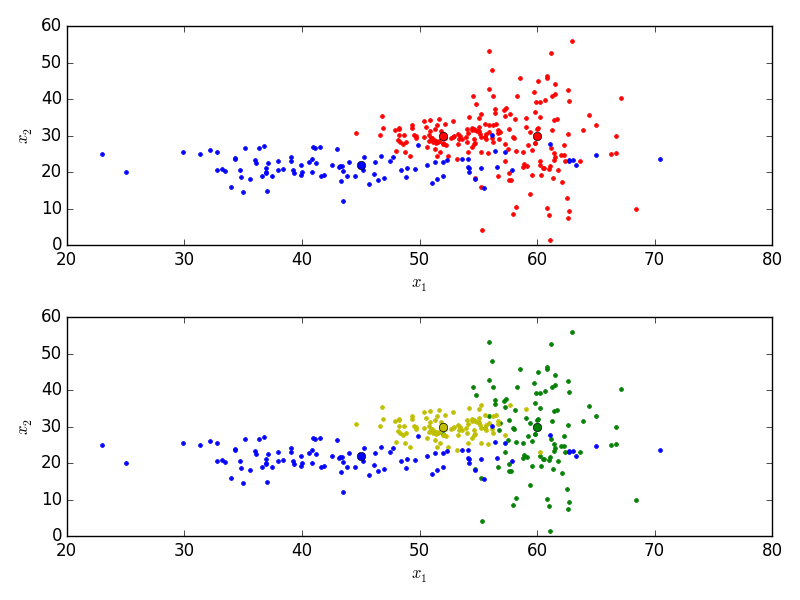
\includegraphics[width=\columnwidth]{samples}
    \caption{Classes 1a (verde), 1b (amarelo) e 2 (azul).}
    \label{fig:samples}
\end{figure}

Pode-se utilizar estas amostras para estimar as probabilidades e densidades de probabilidade desconhecidas. Para problemas de aprendizagem supervisionada, a estimação das $P(\omega_i)$ é bastante simples. Sabendo a frequência relativa de aparição de cada classe $\omega_i$ no conjunto de treinamento, pode-se estimar suas $P(\omega_i)$ (desde que o conjunto de treinamento seja uma boa representação do ``mundo real"). Contudo, estimar as $p(\boldsymbol{x}|\omega_i)$ é complicado quando se tem poucos dados, especialmente quando a dimensionalidade de $\boldsymbol{x}$ aumenta. Uma maneira mais prática é assumir cada $p(\boldsymbol{x}|\omega_i)$ como uma gaussiana, cujas média e matriz de covariância são dadas por $\boldsymbol{\mu}_i$ e $\boldsymbol{\Sigma}_i$. Logo, o problema passa de estimar uma função desconhecida $p(\boldsymbol{x}|\omega_i)$ para estimar os \textbf{parâmetros} $\boldsymbol{\mu}_i$ e $\boldsymbol{\Sigma}_i$.

Para a estimação dos parâmetros, será utilizada a técnica da \textbf{máxima-verossimilhança}.

\subsection{Máxima-Verossimilhança}

Estimação por Máxima-Verossimilhança (Maximum-Likelihood, ML) considera os parâmetros como quantidades cujos valores são fixos, mas desconhecidos. A melhor estimativa de seus valores é aquela que maximiza a probabilidade de obter as amostras observadas. Este método possui uma gama de atributos atrativos. Primeiramente, possui quase sempre boas propriedades de convergência quando o número de amostras de treinamento aumenta. Além disso, ML geralmente é mais simples que métodos alternativos, tais como técnicas bayesianas.

\subsubsection*{Princípio Geral}

Um conjunto $\mathcal{D}$ de amostras é dividido em conjuntos $\mathcal{D}_1, .., \mathcal{D}_c$ cujas amostras são desenhadas independentemente, de acordo com $p(\boldsymbol{x}|\omega_j)$, resultado de variáveis aleatórias independentes e identicamente distribuídas. Assume-se que $p(\boldsymbol{x}|\omega_j)$ tem uma forma paramétrica, como por exemplo $N(\boldsymbol{\mu}_j, \boldsymbol{\Sigma}_j)$, de modo que pode ser escrita como $p(\boldsymbol{x}|\omega_j, \boldsymbol{\theta}_j)$, onde $\boldsymbol{\theta}_j$ consiste nos componentes de $\boldsymbol{\mu}_j$ e $\boldsymbol{\Sigma}_j$. O problema torna-se utilizar as informações dadas pelas amostras para obter boas estimativas dos vetores desconhecidos $\boldsymbol{\theta}_j$, para cada $\omega_j$. Uma simplificação é assumir que as amostras de cada $\mathcal{D}_j$ provêem informações relevantes apenas aos seus respectivos $\boldsymbol{\theta}_j$.

\begin{figure}[ht]
    \centering
    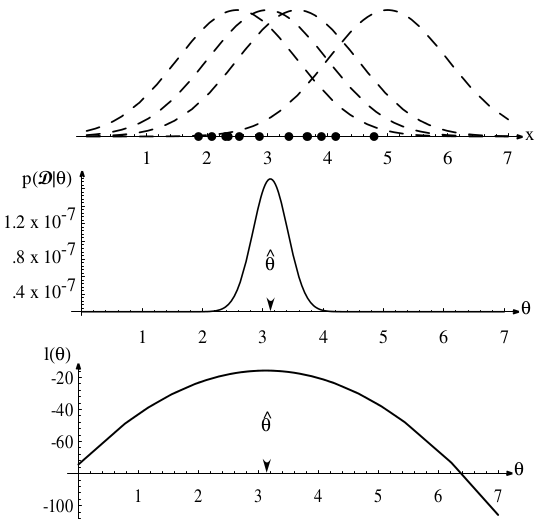
\includegraphics[width=\columnwidth]{maximum-likelihood}
    \caption{Estimação do parâmetro $\boldsymbol{\hat{\theta}}$, o valor $\boldsymbol{\hat{\theta}}$ achado e $l(\boldsymbol{\hat{\theta}})$.}
    \label{fig:maximum-likelihood}
\end{figure}

Usa-se o conjunto $\mathcal{D}$, composto pelas amostras de treinamento $\boldsymbol{x}_1, ..., \boldsymbol{x}_n$ desenhadas independentemente de $p(\boldsymbol{x}|\boldsymbol{\theta})$, para estimar os $\boldsymbol{\theta}$ desconhecidos, tal que

\begin{equation}
    p(\mathcal{D}|\boldsymbol{\theta}) = \prod_{k=1}^{n} p(\boldsymbol{x}_k|\boldsymbol{\theta}).
    \label{eq:pdf_D}
\end{equation}

\noindent A densidade $p(\mathcal{D}|\boldsymbol{\theta})$ é conhecida como a \textbf{verossimilhança} de $\boldsymbol{\theta}$ em relação às amostras, e sua estimativa máxima é, por definição, o valor $\boldsymbol{\hat{\theta}}$ que maximiza  $p(\mathcal{D}|\boldsymbol{\theta})$ (\figureref{maximum-likelihood}).

Devido a ser monotonicamente crescente e mais fácil de trabalhar que a verossimilhança, o uso da log-verossimilhança

\begin{equation}
    l(\boldsymbol{\theta}) \equiv \ln p(\mathcal{D}|\boldsymbol{\theta}) = \sum_{k=1}^{n} \ln p(\boldsymbol{x}_k|\boldsymbol{\theta})
    \label{eq:log_likelihood}
\end{equation}

\noindent é preferível. Logo, a solução para $\boldsymbol{\hat{\theta}}$ é

\begin{equation}
    \boldsymbol{\hat{\theta}} = \arg\max_{\boldsymbol{\theta}} l(\boldsymbol{\theta}),
    \label{eq:hat_theta}
\end{equation}

\noindent onde a dependencia do conjunto de dados $\mathcal{D}$ fica implícito. Se o número de parametros a serem estimados é $p$, então $\boldsymbol{\theta} = (\theta_1, ..., \theta_p)^t$ e $\boldsymbol{\nabla}_{\boldsymbol{\theta}} = (\frac{\partial}{\partial \theta_1}, ..., \frac{\partial}{\partial \theta_p})^t$, e, pela \equationref{log_likelihood}

\begin{equation}
    \boldsymbol{\nabla}_{\boldsymbol{\theta}} l = \sum_{k=1}^{n} \boldsymbol{\nabla}_{\boldsymbol{\theta}} \ln p(\boldsymbol{x}_k|\boldsymbol{\theta}).
    \label{eq:gradient_theta_log}
\end{equation}

Então, um conjunto de condições necessárias para a estimação da máxima verossimilhança para $\boldsymbol{\theta}$ pode ser obtido do conjunto de $p$ equações

\begin{equation}
    \boldsymbol{\nabla}_{\boldsymbol{\theta}} l = \boldsymbol{0}.
    \label{eq:gradient_theta_log_equal_zero}
\end{equation}

Uma solução $\boldsymbol{\hat{\theta}}$ para \equationref{gradient_theta_log_equal_zero} pode ser uma máximo global, um máximo/mínimo local, ou (raramente) um ponto de inflexão de $l(\boldsymbol{\theta})$. Se todas as soluções forem achadas, é garantido que representa o máximo verdadeiro, senão deve-se checar todas as soluções individualmente (ou calcular derivadas de segunda ordem) para identificar qual é o ótimo global.

\subsubsection*{Gaussiana com $\boldsymbol{\mu}$ desconhecido}

Neste caso o vetor $\boldsymbol{\theta} = \boldsymbol{\mu}$, levando a $l(\boldsymbol{\theta}) = l(\boldsymbol{\mu}) \equiv \ln p(\mathcal{D}|\boldsymbol{\mu})$. Logo pela \equationref{log_likelihood},

\begin{equation}
    l(\boldsymbol{\mu}) = \sum_{k=1}^{n} \ln p(\boldsymbol{x}_k|\boldsymbol{\mu}),
    \label{eq:log_mu}
\end{equation}

\noindent e pela \equationref{gradient_theta_log},

\begin{equation}
    \boldsymbol{\nabla}_{\boldsymbol{\mu}} l = \sum_{k=1}^{n} \boldsymbol{\nabla}_{\boldsymbol{\mu}} \ln p(\boldsymbol{x}_k|\boldsymbol{\mu}).
    \label{eq:nabla_mu_log}
\end{equation}

\noindent Como $\boldsymbol{\nabla}_{\boldsymbol{\mu}} \ln p(\boldsymbol{x}_k|\boldsymbol{\mu}) = \boldsymbol{\Sigma}^{-1} (\boldsymbol{x}_k - \boldsymbol{\mu})$ e $\boldsymbol{\nabla}_{\boldsymbol{\mu}} l = 0$ (\equationref{gradient_theta_log_equal_zero}), então

\begin{equation}
    \sum_{k=1}^{n} \boldsymbol{\Sigma}^{-1} (\boldsymbol{x}_k - \boldsymbol{\hat{\mu}}) = \boldsymbol{0}.
    \label{eq:nabla_mu_log_equals_zero}
\end{equation}

\noindent Multiplicando por $\boldsymbol{\Sigma}$ e rearranjando os termos, tem-se

\begin{equation}
    \boldsymbol{\hat{\mu}} = \frac{1}{n} \sum_{k=1}^{n} \boldsymbol{x}_k.
    \label{eq:mu_optimum_case_1}
\end{equation}

Fica evidente que para o caso em que apenas $\boldsymbol{\mu}$ é desconhecido, a estimativa para a máxima verossimilhança é apenas a média das amostras, às vezes escrita como $\boldsymbol{\hat{\mu}}_n$ para clarificar sua dependência do número de amostras.

\subsubsection*{Gaussiana com $\boldsymbol{\mu}$ e $\boldsymbol{\Sigma}$ desconhecidos}

Este é o caso mais típico, quando $\boldsymbol{\mu}$ e $\boldsymbol{\Sigma}$ são desconhecidos. Desta forma, este parâmetros constituem as componentes do vetor paramétrico $\boldsymbol{\theta}$, ou seja $\boldsymbol{\theta} = (\boldsymbol{\mu}, \boldsymbol{\Sigma})^t$. Considerando o caso univariado, $\theta_1 = \mu$ e $\theta_2 = \sigma^2$. Então

\begin{equation}
    \ln p(x_k|\boldsymbol{\theta}) = -\frac{1}{2} \ln 2\pi\theta_2 - \frac{1}{2\theta_2}(x_k - \theta_1)^2
    \label{eq:log_likelihood_mu_sigma_univar}
\end{equation}

\noindent e seu gradiente é

\begin{equation}
    \boldsymbol{\nabla}_{\boldsymbol{\theta}} l = \boldsymbol{\nabla}_{\boldsymbol{\theta}} \ln p(x_k|\boldsymbol{\theta}) = \tworowsmatrix{\frac{1}{\theta_2}(x_k - \theta_1)}{-\frac{1}{2\theta_2} + \frac{(x_k - \theta_1)^2}{2\theta_2^2}}
    \label{eq:grad_log_likelihood_mu_sigma_univar}
\end{equation}

\noindent e pela \equationref{nabla_mu_log_equals_zero} tem-se

\begin{equation}
    \sum_{k=1}^n \frac{1}{\hat{\theta_2}}(x_k - \hat{\theta_1}) = 0
    \label{eq:grad_log_likelihood_mu_sigma_univar_theta_1}
\end{equation}

\noindent e

\begin{equation}
    -\sum_{k=1}^n \frac{1}{2\hat{\theta_2}} + \sum_{k=1}^n \frac{(x_k - \hat{\theta_1})^2}{2\hat{\theta_2}^2} = 0,
    \label{eq:grad_log_likelihood_mu_sigma_univar_theta_2}
\end{equation}

\noindent Rearrumando tudo, tem-se

\begin{equation}
    \hat{\mu} = \frac{1}{n} \sum_{k=1}^n x_k
    \label{eq:mu_optimum_case_2}
\end{equation}

\noindent e

\begin{equation}
    \hat{\sigma}^2 = \frac{1}{n} \sum_{k=1}^n (x_k - \hat{\mu})^2.
    \label{eq:sigma_optimum_case_2}
\end{equation}

Dando um salto de fé (embora esta seja demonstrável, diferente da cristã) e trocando os $\hat{\mu}$ e $\hat{\sigma}$ por $\boldsymbol{\hat{\mu}}$ e $\boldsymbol{\hat{\Sigma}}$, respectivamente, tem-se

\begin{equation}
    \boldsymbol{\hat{\mu}} = \frac{1}{n} \sum_{k=1}^n \boldsymbol{x}_k
    \label{eq:bold_mu_optimum_case_2}
\end{equation}

\noindent e

\begin{equation}
    \boldsymbol{\hat{\Sigma}} = \frac{1}{n} \sum_{k=1}^n (\boldsymbol{x}_k - \boldsymbol{\hat{\mu}})(\boldsymbol{x}_k - \boldsymbol{\hat{\mu}})^t.
    \label{eq:bold_sigma_optimum_case_2}
\end{equation}

\subsection{Análise de Componentes e Discriminantes}

\texttt{TODO} fazer no final, se tiver tempo

\section{Misturas}

\end{document}